%% %%%%%%%%%%%%%%%%%%%%%%%%%%%%%%%%%%%%%%%%%%%%%%%%%%%%%%%%%%%%%%%%%%%%%%%%%%%
%%
%%          $Id: general_rules.tex 420 2013-04-08 15:30:35Z holz $
%%    author(s): RoboCupAtHome Technical Committee(s)
%%  description: description of the GENERAL RULES
%%
%% %%%%%%%%%%%%%%%%%%%%%%%%%%%%%%%%%%%%%%%%%%%%%%%%%%%%%%%%%%%%%%%%%%%%%%%%%%%
\chapter{General Rules \& Regulations}
\label{chap:rules}

These are the general rules and regulations for the competition in the RoboCup@Home league.
Every rule in this section can be considered to implicitly include the term \emph{\enquote{unless stated otherwise}}, meaning that additional or contrary rules in particular
test specifications have a higher priority than those mentioned herein in the general rules and regulations.

%%%%%%%%%%%%%%%%%%%%%%%%%%%%%%%%%%%%%%%%%%%%%%%%%%%%%%%%%
\section{Team Registration and Qualification}


\subsection{Registration and Qualification Process}
\label{rule:participation}

Each year there are four phases in the process toward participation:
\begin{enumerate}
	\item \iterm{Intention of Participation} (optional)
	\item \iterm{Preregistration}
	\item \iterm{Qualification} announcements
	\item Final \iterm{Registration} for qualified teams
\end{enumerate}
Positions 1 and 2 will be announced by a call on the \iterm{RoboCup@Home mailing list}. Preregistration requires a \iterm{team description paper}, a \Term{video}{qualification video} and a \Term{website}{Team Website}.

\subsection{Qualification Video}
As a proof of running hardware, each team has to provide a \iterm{qualification video} showing at least two from the following abilities (minimum requirement):
\begin{itemize}
	\item Human-Robot interaction
	\item Navigation (safe, indoors with obstacle avoidance).
	\item Object detection \& manipulation.
	\item People detection
	\item Speech recognition.
	\item speech synthesis (clear and loud).
\end{itemize}

Showing some of the following abilities is recommended:
\begin{itemize}
	\item Activity recognition
	\item Complex speech recognition
	\item Complex action planning
	\item Gesture recognition
\end{itemize}


Videos should be self-explicative and designed for a general audience, showing the  robot solving complex tasks. The minimum to qualify requires proving the robot is able to solve successfully at least one test of the current or last year's rulebook. For robots moving slowly, we suggest to speed-up videos. When doing so, please specify the speed factor being used (e.g.~2x, 5X, 10X). The same applies for slow motion scenes. Videos should not exceed the average time for a test (max.~\SI{10}{\minute}).

\subsection{Team Website}

The \iterm{Team Website} should be designed for a broader audience, and include scientific material (scientific papers, datasets, and documented open source code). Requirements are as follows:

\begin{enumerate}

	\item \textbf{Multimedia:}~As many photos and videos of the robot(s) as possible.

	\item \textbf{Language:}~The team website has to be in English. Other languages may be also available, but English must be default language.

	\item \textbf{Team:}~Comprehensive list of the team members including brief profiles.

	\item \textbf{RoboCup:}~Link to the league website and previous participation of the team in RoboCup.

	\item \textbf{Scientific approach:}~Include research lines, description of the approaches, and information on scientific achievements.

	\item \textbf{Publications:}~Relevant \iterm{publications} from 5 years up to date. Downloadable publications are scored higher during the qualification process.

	\item \textbf{Open source material:}~Blueprints, datasets, repositories or any kind of contribution to the league is highly scored during qualification process.
\end{enumerate}


\subsection{Team Description Paper}
\label{rule:website_tdp}
The \iaterm{team description paper}{TDP} is an 8-pages long scientific paper which must have a explained description of your main research, including the scientific contribution, goals, scope, and results.

Preferably, it should also contain the following:
\begin{itemize}
	\item the focus of research and the contributions in the respective fields,
	\item innovative technology (if any),
	\item re-usability of the system for other research groups
	\item applicability of the robot in the real world
	\item photo(s) of the robot(s)
\end{itemize}

~\\\noindent As addendum in the 9th page (after references) please include:
\begin{itemize}
	\item Team name
	\item Contact information
	\item Website url
	\item Team members' names
	\item photo(s) of the robot(s), unless included before.
	\item description of the hardware used
	\item Brief, compact list of \iterm{external devices} (See~\refsec{rule:robot_external_computing}), if any.
	\item Brief, compact list of 3rd party reused software packages (e.g.~ROS' \texttt{object\_recognition} should be listed, but not OpenCV).
	\item \textbf{[Open Platform League only]} Brief description of the hardware used by the robot(s).
\end{itemize}

~\\\noindent The TDP has to be in English, up to eight pages in length and formatted according to the guidelines of the RoboCup International Symposium without altering margins or spacing. It goes into detail about the technical and scientific approach.

Please notice that, during qualification process, TDP will be scored by its scientific value, novelty and contributions.


%% %%%%%%%%%%%%%%%%%%%%%%%%%%%%%%%%%%%%%%%
\subsection{Qualification}
\label{rule:qualification}

During the \iterm{qualification process} a selection will be made by the \iaterm{Organizing Committee}{OC} Taken into account and evaluated in this decision process are:
\begin{itemize}
	\item The content on the team website, scoring higher publications and open source resources;
	\item the number of abilities shown in the qualification video,
	\item the complexity of the tasks shown in the qualification video, and
	\item the scientific value, novelty and contributions in the \iterm{team description paper}. %, and
	% \item the information in the \iterm{RoboCup\char64Home Wiki} (added by the team).
\end{itemize}
(Additional) evaluation criteria are:
\begin{itemize}
	\item the performance in previous competitions,
	\item the relevant scientific contributions and publications, and
	\item the contributions to the RoboCup@Home league.
\end{itemize}

\paragraph{Important note to Standard Platform Leagues:} Only unmodified robots may compete in Standard Platform Leagues. Any \textit{slight} modification made to the robot found in the Qualification Material will automatically disqualify the team, for which registration to the international competition will not be possible  (See~\refsec{rule:spl-mods}).

% For getting considered in the evaluation, be sure to insert your team's name when adding information to the \iterm{RoboCup\char64Home Wiki}.


% Local Variables:
% TeX-master: "../Rulebook"
% End:


\section{Audience interaction}
Direct interaction with the audience is not a part of most challenges, though some explicitly require it in an effort to make robots step out of the laboratory.

Informing the audience however is important for the league.
\subsection{Vizbox}
\label{vizbox}

The objective of RoboCup is to \enquote{promote robotics and AI research, by offering a publicly appealing, but formidable challenge} \footnote{\url{http://robocup.org/objective}}.

Part of making RoboCup@Home appealing, is to show the audience what is going on, what the robots should do and what they are doing.

To this end, robots in RoboCup@Home are expected run the RoboCup@Home \href{https://github.com/LoyVanBeek/vizbox}{VizBox}\footnote{\url{https://github.com/LoyVanBeek/vizbox}}.

This is a web server to be run on a robot during a challenge. The page it serves can be displayed on a screen, visible to the audience, via a secondary computer in or around the arena, connected to the web server via the wireless network.

All robots are expected to run the \iterm{VizBox}; the audience expects to know what all the robots are doing and what each challenge entails.

The \iterm{VizBox}'s code is hosted \url{https://github.com/LoyVanBeek/vizbox}.
We want to show the audience a consistent presentation, so ideally, all teams run the same VizBox code.
Sharing your changes back in the form of a Pull Request is much appreciated so all teams can benefit.

The \iterm{VizBox} has the following visualization capabilities:
\begin{itemize}
	\item Images of what the robot sees or a visualization of the robot's world model, eg. camera images, it's map, anything to make clear what is going on to the audience.
	\item Show an outline of the current challenge and where the robot is in the story of the current challenge.
	\item Subtitles of what the robot and operator just said; their conversation
\end{itemize}

Additionally, the \iterm{VizBox} offers a way to \textbf{input} a text command to the robot, to bypass automatic speech recognition if need be.

The exact documentation is maintained in the repository of the \iterm{VizBox} itself.

%%%%%%%%%%%%%%%%%%%%%%%%%%%%%%%%%%%%%%%%%%%%%%%%%%%%%%%%%
\section{Scenario}
\label{sec:scenario}

The tests take place in the \iterm{RoboCup@Home arena}. Nonetheless, some tests can take place outside the arena, in a previously unknown public place. Rules in this section are related to the \iterm{RoboCup@Home arena} and its contents.

\subsection{RoboCup@Home arena}
The \iterm{RoboCup@Home arena} is a realistic home setting (apartment) consisting of inter-connected rooms.
The minimal configuration consists of
\begin{itemize}
	\item bedroom,
	\item dining room,
	\item living room, and
	\item kitchen.
\end{itemize}
Depending on the Local Organization, there may be multiple apartments which may be different to each other.
Robot must be prepared to perform any task in any arena, not the same arena every time.

The arena is decorated and dressed to resemble a typical apartment in the hosting country, including all necessities and decorations one can find in a normal house.
Please do note that what is considered as \enquote{normal} may greatly vary by culture and on the location where the RoboCup event is hosted.
Decorations include, but are not limited to: plants, mirrors, paintings, posters, plates, picture frames, wall clocks, candles with holders, and books.
For a description of objects, please refer to \refsec{rule:scenario_objects}

\subsection{Walls, doors and floor}
\label{rule:scenario_walls}

The indoor home setting will be surrounded by high and low \Term{walls}{Arena walls}.
These walls will be built up using standard fair construction material.

\begin{enumerate}
	\item \textbf{Walls:} Walls have a minimum height of \SI{60}{\centi\meter}. A maximum height is not specified, but must allow the audience to watch the competition.\\
	Walls are fixed and not to be modified during the competition (see~\refsec{rule:scenario_changes}).

	\item \textbf{Doors:} There will be at least two \Term{doors}{Arena doors}, an entrance and an exit, to be used as starting points for the robots (see~\refsec{rule:start_position}).
	% At least one of the entrances will be a door with a handle (not a knob).\
	Inside the arena rooms are connected by doors (at least one).
	All doors have handles, not knobs.
	Doors can be closed at any time, and it is expected that robots be able to open them.

	\item \textbf{Floor:} The floor of the arena as well as the doorways of the arena are even.
	That is, there will be no significant steps or even stairways.
	However, minor unevenness such as carpets, transitions in floor covering between different areas, and minor gaps (especially at doorways) can be expected.

	\item \textbf{Appearance:} Floor and walls are mainly uni-colored but can contain texture, e.g., a carpet on the floor, or a poster or picture on the wall.\\
	Although being unlikely at the moment, transparent elements are also possible.
\end{enumerate}


\subsection{Furniture}
\label{rule:scenario_furniture}
The arena will be equipped with typical objects (furniture) that are not specified in quantity and kind.

The minimal configuration consists of:
\begin{itemize}
	\item a bed,
	\item a couch,
	\item a small table,
	\item a small dinner table with two chairs,
	\item an open cupboard or small table with a television and remote control,
	\item a cupboard with drawers, and
	\item a bookcase or shelf with doors and some books inside
\end{itemize}

Likewise the arena's kitchen must have:
\begin{itemize}
	\item a dishwasher,
	\item a microwave,
	\item a sink, and
	\item a refrigerator in the kitchen (with some cans and plastic bottles inside).
\end{itemize}

A typical arena setup is shown in~\reffig{fig:scenario_arena}.

\begin{figure}[tbp]
	\centering
	\subfloat[Typical arena]{\label{fig:scenario_arena}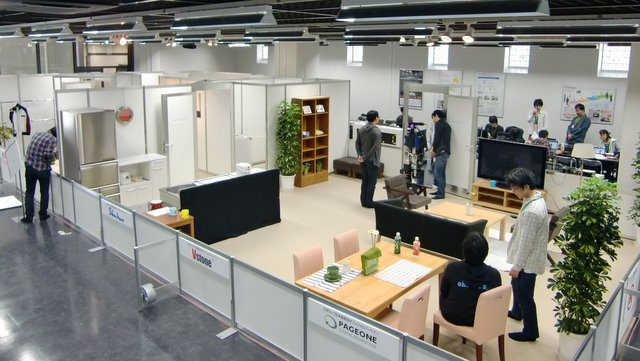
\includegraphics[height=46mm]{images/typical_arena.jpg}} ~
	\subfloat[Typical objects]{\label{fig:scenario_objects}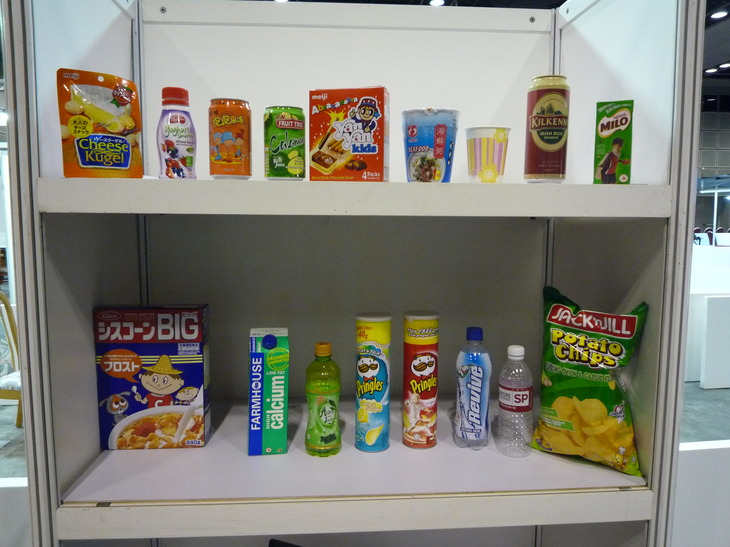
\includegraphics[height=46mm]{images/typical_objects.jpg}}
	\caption{Scenario examples: (a) a typical arena, and (b) typical objects.}
	\label{fig:arena}
\end{figure}


\subsubsection{Cupboard}
The cupboard can be any shelf-like furniture in which objects can be placed.
\begin{itemize}
	\item[\textbf{Doors:}] The cupboard may have doors.
	\item[\textbf{Drawers:}] The cupboard must have at least two drawers betweem 90cm and 120cm from floor level.
	\item[\textbf{Shelves:}] The minimum distance between shelf or layers is 30cm.
\end{itemize}

\subsubsection{Shelf}
A shelf, rack, or bookcase is required in RoboCup@Home.
The shelf can be any shelf-like furniture in which objects can be placed.
\begin{itemize}
	\item[\textbf{Doors:}] The shelf must have at least one door (preferrably a vertical one) covering up to one half of it.
	\item[\textbf{Drawers:}] The shelf must have no drawers.
	\item[\textbf{Shelves:}] The shelf must have 5 shelves or layers between 0.0m and 1.80m from the ground, with a minimum distance of 30cm between shelves or layers.
\end{itemize}

\subsubsection{Fridge}
Fridges must not be smaller than 120m. At least one powered and functioning fridge is required.


\subsection{Changes to the arena}
\label{rule:scenario_changes}

Since the robots should be able to function in the real world the scenario is not fixed and might change without further notice.
\begin{enumerate}
	\item \textbf{Major changes:}
	The arena is meant to be a simulated apartment.
	The furniture might be moved around between tests.
	This includes furniture that is a named location (see~\refsec{rule:scenario_names}).
	As in a normal home, furniture is not very likely to move from one room to another and is unlikely to be moved to the other side of a room.
	However, a couch or table may be rotated, moved to its side etc.
	Walls will stay in place and rooms will not change function.
	Passages might be blocked and cleared.
	One hour before a test slot begins no \iterm{major changes} will be made.
	This time will be shortened in the future.

	\item \textbf{Minor changes:} In contrast to major changes, \iterm{minor changes} like, for instance, slightly moved chairs cannot be avoided and may happen at any time (even during a test).
\end{enumerate}


%%%%%%%%%%%%%%%%%%%%%%%%%%%%%%%%%%%%%%%%%%%%%%%%%%%%%%%%%%%%%%%%%%
%
% Objects section.
%
% Revisited by Mauricio Matamoros for 2015
%
%%%%%%%%%%%%%%%%%%%%%%%%%%%%%%%%%%%%%%%%%%%%%%%%%%%%%%%%%%%%%%%%%%
\def\NumObjects{30\ }
\def\NumLocations{20\ }
\def\NumNames{20\ }

\subsection{Objects}
\label{rule:scenario_objects}
Some tests in the RoboCup@Home league involve recognizing and manipulating \iterm{objects}(See~\reffig{fig:scenario_objects}).
The TC will compile a list of at least \NumObjects objects for this purpose, assigning them official names.
Most objects are likely to be lightweight and easy to grasp with one hand.
Each object has assigned a category (e.g. an \textit{apple} and a \textit{banana} belong to the \textit{fruits} category).
Each \iterm{object category} has assigned a \iterm{predefined location} (e.g. an \textit{fruits} can be found in the \textit{kitchen table}).
Assignments are announced during setup days (See~\refsec{chap:setup_and_preparation}).
An exemplar of each object is provided before the competition for training.

There are two types of objects:

\begin{enumerate}
	\item \textbf{\iterm{Known objects}:} Objects previously known by the robot and that it can identify and manipulate.
	There are two kinds of known objects:
	\begin{enumerate}
		\item \textbf{\iterm{Regular objects}:} Objects with no noticeable difference among peers (e.g.~soda can, cereal box, cutlery, etc).
		\item \textbf{\iterm{Alike objects}:} Objects which are different one from another, but still considered by people to be the same (e.g.~apple, sandwich, cloth, etc.).
	\end{enumerate}

	\item \textbf{\iterm{Unknown objects}:} Any other object that is not known beforehand but can be grasped or handled.
\end{enumerate}

\subsection{List of Predefined Objects}
\label{rule:scenario_objects_list}
The minimal configuration consists of:
\begin{itemize}
	\item \textbf{\iterm{Tableware}:} Dish, bowl, cup (or mug), and napkin.
	\item \textbf{\iterm{Cutlery}:} Fork, knife, and spoon.
	\item \textbf{\iterm{Bags}:} Lightweight. With stiff, vertical handles.
	\item \textbf{\iterm{Trays}:} A transport object like a tray or basket. Intended for two-handed manipulation.
	\item \textbf{\iterm{Pourable}:} An object whose content can be poured (e.g. muesli, cereal, etc.).
	\item \textbf{\iterm{Heavy object}:} Weight between 1.0kg and 1.5kg).
	\item \textbf{\iterm{Tiny object}:} A lightweight object with no bigger than 5cm (e.g. paper, teabag, pen).
	\item \textbf{\iterm{Fragile object}:} An easy-to-break object, (e.g. chocolate egg).
	\item \textbf{\iterm{Amorphous object}:} An flexible object that may take an infinite number of shapes (e.g. cloth, magnetic puzzle, etc.).
\end{itemize}

\paragraph*{Important note:} It is not allowed to modify any of the objects provided for training.
Teams are not allowed to keep more than 5 the objects provided for training at a time nor retaining it for more than one hour.

\begin{figure}[H]
	\centering
	\subfloat[Bright-colored paper bags]{
		\label{fig:scenario_container_bag}
\includegraphics[width=0.33\textwidth]{images/container_paper_bag.png}}~
	\subfloat[Cereal bowls]{
		\label{fig:scenario_container_bowl}
\includegraphics[width=0.33\textwidth]{images/container_bowl.png}}~
	\subfloat[Serving tray]{
		\label{fig:scenario_container_tray}
\includegraphics[width=0.33\textwidth]{images/container_tray.png}}
	\caption{Example of object containers}
	\label{fig:scenario_containers}
\end{figure}

\subsection{Attributes of Predefined Objects}
\label{rule:scenario_objects_attributes}
During the competition, objects can be requested based on their category \iterm{object category}, its physical attributes, or a combination of both.
Relevant attributes to be used are:
\begin{itemize}
	\item Color (e.g. red, blue, black with white dots, etc.).
	\item Relative estimated size (smallest, largest, big one, etc.).
	\item Relative estimated weight (lightest, heaviest).
	\item Relative position (left of, right most, etc.).
	\item Object description (is fragile, is container, can be poured, requires two hands, etc.).
\end{itemize}

\noindent\textbf{Remark:} Measurements are estimations and based on common sense. It is OK for robots to consider similar objects to be about the same size or weight.

%%%%%%%%%%%%%%%%%%%%%%%%%%%%%%%%%%%%%%%%%%%%%%%%%%%%%%%%%%%%%%%%%%
%
% Predefined locations section.
%
%%%%%%%%%%%%%%%%%%%%%%%%%%%%%%%%%%%%%%%%%%%%%%%%%%%%%%%%%%%%%%%%%%

\subsection{Predefined rooms and locations}
\label{rule:scenario_locations}
Some tests in the RoboCup@Home league involve \iterm{predefined locations} where people or objects can be found.
The TC will compile a list of predefined locations that may include furniture (e.g. bookshelf), decorations (e.g. plant, mirror), and doors.
Each \iterm{predefined location} has assigned a \iterm{location class} (e.g. an \textit{coach} and a \textit{arm chair} belong to the \textit{seat} class).
Room names, predefined locations, and location classes are announced during setup days (See~\refsec{chap:setup_and_preparation}).



\subsection{Predefined (person) names}\label{rule:scenario_names}
Some tests in the RoboCup@Home league involve memorizing a person name.
All people in the arena has an assigned \iterm{predefined name}.
The TC will compile a list of \NumNames \iterm{predefined names}.
The names are \SI{25}{\percent} male, \SI{25}{\percent} female, and \SI{50}{\percent} gender-neutral, taken from the list of most common used names in the United States.
Predefined names are announced during setup days (See~\refsec{chap:setup_and_preparation}).


\subsection{Wireless network}
\label{rule:scenario_wifi}

For wireless communication, an \iterm{arena network} is provided. The actual infrastructure depends on the local organization.
The organizers do NOT guarantee reliability and performance of wireless communication.
Teams required to start must do so regardless the availability of the network infrastructure.

The following rules apply:

\begin{itemize}
	\item Only the \iterm{arena network} can be used during tests.
	\item During the competitions, only the active team is allowed to use the \iterm{arena network}.
	\item The \iterm{arena network} provides one Virtual Local Area Networks (VLANs) per team.
	\item Each VLAN is most likely to have its own SSID/password.
	\item VLAN traffic is separated from any other team, routed to the team's network cable (team area).
	\item Each VLAN is also connected to the Internet.
\end{itemize}

\indent\textbf{Remark:} Teams broadcasting unauthorized (aka rogue) wireless networks will be disqualified from the competition, and have their devices confiscated by the OC.
This includes smartphones and concealed SSIDs.
It is advised to verify your devices.


% Local Variables:
% TeX-master: "../Rulebook"
% End:


%%%%%%%%%%%%%%%%%%%%%%%%%%%%%%%%%%%%%%%%%%%%%%%%%%%%%%%%%
\section{Robots}
\label{rule:robots}

\subsection{Number of robots}
\label{rule:robots_number}

\begin{enumerate}
	\item \textbf{Registration:} The maximum \term{number of robots} per team is \emph{two} (2).
	\item \textbf{Regular Tests:} Only one robot is allowed per test. For different tests different robots can be used.
	% \item \textbf{Open Demonstrations:} In the \iterm{Open Challenge} and the \iterm{Finals} both robots can be used simultaneously.
\end{enumerate}

\subsection{Appearance and safety}
\label{rule:robot_appearance}

Robots should have a nice product-like appearance, be safe to operate, and should not annoy people. The following rules apply to all robots and are part of the \iterm{Robot Inspection} test (see~\refsec{sec:robot_inspection}).
\begin{enumerate}
	\item \textbf{Cover:} The robot's internal hardware (electronics and cables) should be covered in an appealing way. The use of (visible) duct tape is strictly prohibited.
	\item \textbf{Loose cables:} Loose cables hanging out of the robot are not permitted.
	\item \textbf{Safety:} The robot must not have sharp edges or elements that might harm people.
	\item \textbf{Annoyance:} The robot must not be continuously making loud noises or use blinding lights.
	\item \textbf{Marks:} The robot may not exhibit any kind of artificial marks or patterns.
	\item \textbf{Driving:} To be safe, the robots should be careful when driving (obstacle avoidance is mandatory).
\end{enumerate}

\subsection{Standard Platform Leagues}
RoboCup@Home features two Standard Platform Leagues adhering to the rules listed above.

\subsubsection{Modifications}
\label{rule:spl-mods}
Standardized platforms allow teams to compete in equality of conditions by eliminating all hardware-dependent variables.
Therefore, modifications and alterations to the robots are strictly forbidden; including, but not limited to attaching, connecting, plugging, gluing, and taping components into and onto the robot, as well as modifying or altering the robot structure.
Voiding this rule leads to immediate disqualification from the competition and penalty for the team (see~\refsec{rule:extraordinary_penalties}).

During the \iterm{Robot Inspection} test (see~\refsec{sec:robot_inspection}), the TC will verify that the robot is in proper state for the competition; presenting no alterations and a neat condition.
EC and TC members may request re-inspection of a SPL robot at any time during the competition.

\textbf{Clothing, coloring, and stickers:} Robots are allowed to \enquote{wear} clothes, as well as have stickers (e.g., a sticker exhibiting the logo of an sponsor).
Painting the robot with another color or design is also allowed. 
However, artificial markers (e.g. bar codes, QR codes, OpenCV markers) are strictly forbidden. 
Teams should contact the robot providet before altering the robot's appearance.

% \subsubsection{Domestic Standard Platform League}
% The characteristics of the Toyota Human Support Robot are detailed below.

% \begin{itemize}
	% \item Aimed at human support tasks, elderly care et cetera
	% \item Omni-directional base, maximum speed 0.8km/h
	% \item 1 arm with multifunctional gripper through a vacuum pad. The wrist is equipped with a force-torque sensor. Capable of lifting 1.2kg.
	% \item RGB-D, stereo cameras and wide-angle camera
	% \item Display mounted in head, separate tablet interface
	% \item Access to cloud-based services
	% \item Equipped with a microphone array
	% \item Gravity compensated arm
	% \item Height-adjusting torso
% \end{itemize}
% 
% \subsubsection{Social Standard Platform League}
% The characteristics of the Softbank Robotics/Aldebaran Pepper are detailed below.
% 
% \begin{itemize}
	% \item Aimed at social interaction, public environments, explainable artificial intelligence
	% \item Omni-directional base, maximum speed 3km/h
	% \item 2 arms mostly intended for social gesturing.
	% \item 3D and 2 HD cameras
	% \item Equipped with a built-in tablet
	% \item Access to cloud-based services
	% \item Equipped with a 4-microphone array in the head
	% \item Emotion recognition by voice and images
	% \item Emotion engine to adapt it's attitude
% \end{itemize}

\subsection{Robot Specifications for the Open Platform League }
Robots competing in the RoboCup@Home Open Platform League must comply with security specifications in order to avoid causing any harm while operating in human environments.

\subsubsection{Size and weight of robots}
\label{rule:robots_size}

\begin{enumerate}
	\item \textbf{Dimensions:} The dimensions of a robot should not exceed the limits of an average door, which is \SI{200}{\centi\meter} by \SI{70}{\centi\meter} in most countries.\\
	The TC may allow the qualification and registration of larger robots, but due to the international character of the competition it cannot be guaranteed that the robots can actually enter the arena. In case of doubt, contact the local organization.
	\item \textbf{Weight:} There is no specific weight restriction. However, the weight of the robot and the pressure it exerts on the floor should not exceed local regulations for the construction of buildings which are used for living and/or offices in the country where the competitions is being held.
	\item \textbf{Transportation:} Team members are responsible for quickly moving the robot out of the arena.	If the robot cannot move by itself (for any reason), the team members must be able to transport the robot away with an easy and fast procedure.
\end{enumerate}



\subsubsection{Emergency stop button}
\label{rule:robots_emergency_button}

\begin{enumerate}
	\item \textbf{Accessibility and visibility:} Every robot has to provide an easily accessible and visible \iterm{emergency stop} button.
	\item \textbf{Color:} It must be coloured red, and be the only red button on the robot.
	The TC may ask the team to tape over or remove any other red button present in the robot.
	\item \textbf{Robot behavior:} When the \iterm{emergency stop} button is pressed, the robot and all its parts must stop moving immediately.
	\item \textbf{Inspection:} The emergency stop button is tested during the \iterm{Robot Inspection} test (see~\refsec{sec:robot_inspection}).
\end{enumerate}




\subsubsection{Start button}
\label{rule:start_button}

\begin{enumerate}
	\item \textbf{Requirements:} As stated in~\refsec{rule:start_signal}, teams that aren't able to carry out the default start signal (opening the door) have to provide a \iterm{start button} that can be used to start tests.
	Teams need to announce this to the TC before every test that involves a start signal, including \iterm{Robot Inspection}.

	\item \textbf{Definition:} The start button can be any \enquote{one-button procedure} that can be easily executed by a referee (e.g. releasing of the \iterm{emergency button} (\refsec{rule:robots_emergency_button}), a green button, or a software button in a Graphical User Interface).
	\item \textbf{Inspection:} The start button is tested during the the \iterm{Robot Inspection} test (see~\refsec{sec:robot_inspection}).
\end{enumerate}




% \subsubsection{Audio output plug}
% \label{rule:roobt_audio_out}

% \begin{enumerate}
% 	\item \textbf{Mandatory plug:} Either the robot or some external device connected to it \emph{must} have a \iterm{speaker output plug}. It is used to connect the robot to the sound system so that the audience and the referees can hear and follow the robot's speech output.
% 	\item \textbf{Inspection:} The output plug needs to be presented to the TC during the \iterm{Robot Inspection} test (see~\refsec{sec:robot_inspection}).
% 	\item \textbf{Audio during tests:} Audio (and speech) output of the robot during a test have to be understood at least by the referees and the operators.
% 	\begin{compactitem}
% 		\item It is the responsibility of the teams to plug in the transmitter before a test, to check the sound system, and to hand over the transmitter to next team.
% 		\item Do not rely on the sound system! For fail-safe operation and interacting with operators make sure that the sound system is not needed, e.g., by having additional speakers directly on the robot.
% \end{compactitem}
% \end{enumerate}




\subsubsection{Appearance}
\label{rule:robots_appearance}
Open Platform Robots should have a neat appearance that resembles more a safe and finished product than an early stage prototype, paying special attention in completely cover the robot's internal hardware (electronics and cables) in an appealing way.
% However, teams must keep in mind that no artificial markers are allowed when personalizing the appearance or a robot. This includes, but is not limited to bar codes, QR codes, OpenCV markers, fluorescent and phosphorescent colors, and reflective stickers.
Although covering the robot's internal hardware with a T-Shirt is not forbidden (for now) it is strongly unadvised.



% Local Variables:
% TeX-master: "../Rulebook"
% End:


% %% %%%%%%%%%%%%%%%%%%%%%%%%%%%%%%%%%%%%%%%%%%%%%%%%%%%%%%%%%
% 
% External Devices
% 
% %% %%%%%%%%%%%%%%%%%%%%%%%%%%%%%%%%%%%%%%%%%%%%%%%%%%%%%%%%%

\section{External devices}
\label{rule:robot_external_devices}
Everything which is not part of the robot is considered an \iterm{external device}.
All external devices must be authorized by the \iaterm{Technical Committee}{TC} during the \iterm{Robot Inspection} test (see~\refsec{sec:robot_inspection}).
The \iaterm{Technical Committee}{TC} specifies whether an external device can be used freely, under referee supervision, and its impact on scoring.
In general, external devices must be removed quickly after the test.
	
\noindent \textbf{Remark:} The use of \iterm{wireless devices} is strictly prohibited. \iterm{External microphones}, hand microphones, and headsets are not allowed in OPL and it use is discouraged in DSPL and SSPL.

\subsection{On-site external computing}
Computing resources that are not physical attached to the robot are considered \iterm{external computing resources}.
The use of up to 5 external computing resources is allowed, but only through the arena network (see \refsec{rule:scenario_wifi}) and with the previous approval of the \iaterm{Technical Committee}{TC}.
Teams must announce the use of any external computing resource at least 1 month before the competition to the \iaterm{Technical Committee}{TC}.

External Computing Devices must be placed in the \iaterm{\textbf{E}xternal \textbf{C}omputing \textbf{R}esource \textbf{A}rea}{ECRA} which is announced by the \iaterm{Technical Committee}{TC} during setup days.
A switch connected to the arena wireless network will be available to teams in the ECRA.
It is strictly forbidden to connect any kind of device or peripheral (e.g. screens, mouses, keyboards, etc.) to the computers in the ECRA during the competition.

A maximum of two laptops and two people from different teams is allowed at any time in the ECRA.
Teams using laptops as External Computing Devices must remove the device immediately after the test.
Once a test has started, all people must stay at least 1 meter from the ECRA.
Interacting with computers in the ECRA after the Referee has given the start signal will cause the immediate disqualification of the team.

\noindent \textbf{Remark:} Robot operation must be able to operate safely when \iterm{external computing resources} are unavailable.



% On-line devices
\subsection{On-line external computing}
\label{rule:robot_external_computing_online}
Robots are allowed to use \enquote{Cloud services}, \enquote{Internet API's}, and any other type of \iterm{external computing resource}.
Same restrictions for on-site external computing resources apply.

\noindent \textbf{Remark:} The competition organization doesn't guarantee or take any responsibility regarding the availability or reliability of neither the network nor Internet connection.
Teams' use of external computing resources is at their own risk.



% DSPL laptop
\subsection{Official Standard Laptop for DSPL}
\label{rule:osl_dspl}

In the Domestic Standard Platform League, teams may use the \iaterm{Official Standard Laptop}{OSL} connected to the Toyota HSR via Ethernet cable, safely located in the TOYOTA HSR \iterm{Mounting Bracket} provided by TOYOTA for this purpose.

\subsubsection{Technical Specifications}
The technical specifications for the Official Standard Laptop in the Domestic Standard Platform League are the following:


 \begin{itemize}
  \item \textbf{Brand and model:} DELL Alienware 15 or 17
  \item \textbf{CPU:} Core-i7 series
  \item \textbf{RAM:} 16GB or 32GB
  \item \textbf{GPU:} NVIDIA GeForce GTX 1070 or 1080
  \item \textbf{Storage:} Unrestricted.
\end{itemize}

No other brands or models will be accepted. There are no constrains regarding the software installed in the OSL but no additional hardware is allowed.

The referees, Technical Committee, and Organizing Committee members may run random checks anytime during the competition prior to the test to verify that the laptop in the TOYOTA HSR \iterm{Mounting Bracket} has no additional hardware plugged in, and matches the authorized specifications.


% Local Variables:
% TeX-master: "../Rulebook"
% End:


%%%%%%%%%%%%%%%%%%%%%%%%%%%%%%%%%%%%%%%%%%%%%%%%%%%%%%%%%
\section{Organization of the competition}
\label{sec:procedure_during_competition}

\subsection{Stage system}\label{rule:stages}

The competition features a \iterm{stage system}. It is organized in two stages each consisting of a number of specific tasks. It ends with the \iterm{Finals}.

Each \iaterm{stage} comprehends a set of tasks grouped in two thematic scenarios.
% \iaterm{House Cleaner} and \iaterm{Party Host}.
The \iaterm{House Holder} scenario features tasks related to cleaning, organizing, and giving maintenance; while the \iaterm{Party Host} scenario focuses in attending guests needs and providing general assistance during a party.

\begin{enumerate}
	\item \textbf{Robot Inspection:} For security, robots are inspected during setup days. A robot must pass \iterm{Robot Inspection} test (see~\refsec{sec:robot_inspection}) in order to compete.

	\item \textbf{Stage~I:} The first days of the competition called \iterm{Stage~I}.
	All qualified teams can participate in \iterm{Stage~I}.
	The same task can be performed multiple times (See~\refsec{rule:score_system}).

	\item \textbf{Stage~II:} The best \emph{50\% of teams}\footnotemark (after Stage~I) advance to \iterm{Stage~II}.
	Here, tasks require more complex abilities or combinations of abilities.\\
	\footnotetext{If the total number of teams is less than 12, up to 6 teams may advance to Stage~II}
	The \iterm{Open Challenge} is the open demonstration in Stage~II.

	\item \textbf{Final demonstration:} The best \emph{two teams} of each league, the ones with the highest score after Stage~II, advance to the final round.
	The final round features only a single task integrating all tested abilities.
	In order to participate in the Finals, a team must have solved at least one task of the Stage~II.
\end{enumerate}

In case of having no considerable score deviation between a team advancing to the next stage and a team dropping out, the TC may announce additional teams advancing to the next stage.


%%%%%%%%%%%%%%%%%%%%%%%%%%%%%%%%%%%%%%%%%%%%%%%%%%%%%%%%%
\subsection{Schedule}
\label{rule:schedule}

\begin{enumerate}
	\item \textbf{Thematic scenario blocks:} Each \iterm{thematic scenario} or \iterm{theme} is split in two \iterm{blocks}.
	At least two blocks are scheduled per day, having each block an assigned theme and lasting no less than two hours.
	The \iaterm{Organizing Committee}{OC} announces the schedule during the setup days (see Table \ref{tbl:schedule}).

	\item \textbf{Slots:} The \iaterm{Organizing Committee}{OC} assigns at least two \iterm{test slots} of 5 minutes to each team in each block.
	A team can solve any task during its test slot.
	Remaining block time can be used to assign additional testing slots to interested teams.
	Testing slots are randomly assigned to teams in each block.

	\item \textbf{Tests:} Teams must inform the OC in advance which task(s) will try to solve.
	Only one task can be attempted per test slot.

	\item \textbf{Participation is default:} Teams have to indicate to the \iaterm{Organizing Committee}{OC} when they are \emph{skipping} a test slot. Without such indication, they may receive a penalty when not attending (see~\refsec{rule:not_attending}).
\end{enumerate}

% Please add the following required packages to your document preamble:
% \usepackage[table,xcdraw]{xcolor}
% If you use beamer only pass "xcolor=table" option, i.e. \documentclass[xcolor=table]{beamer}
\begin{table}[h]
	\centering\small
	\newcommand{\teams}[3]{%
		\tiny
		\begin{tabular}{c}%
			\textit{Test slot 1, team $#1$}\\
			\textit{Test slot 2, team $#2$}\\
			$\vdots$\\
			\textit{Test slot $n$, team $#3$}\\
		\end{tabular}
	}
	\newcommand{\wcell}[2]{%
		\parbox[c]{2.5cm}{%
			\vspace{#1}%
			\centering%
			#2%
			\vspace{#1}%
		}%
	}
	\newcommand{\cell}[1]{\wcell{0.2\baselineskip}{#1}}


	\begin{tabular}{
		>{\centering\arraybackslash}m{2.5cm}|%
		>{\columncolor[HTML]{9AFF99}}c |%
		>{\columncolor[HTML]{9AFF99}}c |%
		>{\columncolor[HTML]{CBCEFB}}c |%
		>{\columncolor[HTML]{CBCEFB}}c |%
	}
	\multicolumn{1}{ c }{}
		& \multicolumn{1}{ c }{\cellcolor{white} Day 1 }
		& \multicolumn{1}{ c }{\cellcolor{white} Day 2 }
		& \multicolumn{1}{ c }{\cellcolor{white} Day 3 }
		& \multicolumn{1}{ c }{\cellcolor{white} Day 4 }
		\\\cline{2-5}
	\cell{Block 1\\\footnotesize(9:00 - 12:00)}
		& \cell{House Holder\\\teams{i}{j}{i}}
		& \cell{Party Host\\\teams{k}{i}{k}}
		& \cell{House Holder\\\teams{i}{j}{i}}
		& \cell{Party Host\\\teams{j}{k}{j}}\\\cline{2-5}

	\multicolumn{1}{ c }{}
		& \multicolumn{4}{ c }{\wcell{0.5\baselineskip}{\color{gray}Lunch}}\\\cline{2-5}

	\cell{Block 2\\\footnotesize(9:00 - 12:00)}
		& \cell{House Holder\\\teams{i}{k}{i}}
		& \cell{Party Host\\\teams{k}{j}{k}}
		& \cell{Party Host\\\teams{i}{i}{k}}
		& \cell{House Holder\\\teams{k}{j}{j}}\\\cline{2-5}

	\multicolumn{1}{ c }{}
		& \multicolumn{2}{ c }{\wcell{0.5\baselineskip}{\color[HTML]{029734}Stage 1}}
		& \multicolumn{2}{ c }{\wcell{0.5\baselineskip}{\color[HTML]{6668e5}Stage 2}}\\
	\end{tabular}

	\caption{Example schedule.
		Each team has assigned at least two test slots in every block.
		At least two blocks are scheduled per day with an assigned theme.
		A team can choose a different task in each test, meaning at least 4 different tests per stage.
	}
	\label{tbl:schedule}
\end{table}


\subsection{Score system}
\label{rule:score_system}
Each task has a main objective and a set of scoring bonuses.
To score in a test, a team must successfully accomplish the main objective of the task; bonuses are not considered otherwise.
Overall scoring is calculated as the sum of the maximum score obtained in each ability.

The \iaterm{score system} has the following constrains
\begin{enumerate}
	\item \textbf{Stage~I:} The maximum total score per task in \iterm{Stage~I} is \scoring{1000 points}.
	
	\item \textbf{Stage~II:} The maximum total score per task in \iterm{Stage~I} is \scoring{2000 points}.

	\item \textbf{\iterm{Finals}:} Final score is normalized and a special evaluation is used.

	\item \textbf{Minimum score:} The minimum total score per test in \iterm{Stage~I} and \iterm{Stage~II} is \scoring{0 points}.
	Teams cannot receive negative points.

	\item \textbf{Penalties:} An exception to \emph{minimum score} rule are penalties.
	Both penalties for not attending (see~\refsec{rule:not_attending}) and extraordinary penalties (see~\refsec{rule:extraordinary_penalties}) can cause a total negative score.
\end{enumerate}




% Local Variables:
% TeX-master: "../Rulebook"
% End:


%%%%%%%%%%%%%%%%%%%%%%%%%%%%%%%%%%%%%%%%%%%%%%%%%%%%%%%%%
\section{Procedure during Tests}

\subsection{Safety First!}
\label{rule:safetyfirst}
\begin{enumerate}
	\item \textbf{Emergency Stop:} At any time when operating the robot inside and outside the scenario the owners have to stop the robot immediately if there is a remote possibility of dangerous behavior towards people and/or objects.
	\item \textbf{Stopping on request:} If a referee, member of the Technical or Organizational committee, an Executive or Trustee of the federation tells the team to stop the robot, there will be no discussion and the robot has to be stopped \emph{immediately}.
	\item \textbf{Penalties:} If the team does not comply, the team and its members will be excluded from the ongoing competition immediately by a decision of the RoboCup@Home \iaterm{Technical Committee}{TC}. 	Furthermore, the team and its members may be banned from future competitions for a period not less than a year by a decision of the RoboCup Federation Trustee Board.
\end{enumerate}

\subsection{Maximum number of team members}
\label{rule:number_of_people}
\begin{enumerate}
	\item \textbf{Regular Tests:} During a regular test, the maximum number of team members allowed inside the arena is \emph{one} (1).
	Exceptions are tests that explicitly require volunteer assistance.
	\item \textbf{Setup:} During the setup of a test, the number of team members inside the arena is not limited.
	\item \textbf{Moderation:} During a regular test, one team member \emph{must} be available to host and comment the test (see~\refsec{rule:moderator}).
\end{enumerate}

\subsection{Fair play}
\label{rule:fairplay}
\iterm{Fair Play} and cooperative behavior is expected from all teams during the entire competition, in particular:
\begin{itemize}
	\item while evaluating other teams,
	\item while refereeing, and
	\item when having to interact with other teams' robots.
\end{itemize}
This also includes:
\begin{itemize}
	\item not trying to cheat (e.g.~pretending autonomous behavior where there is none),
	\item not trying to exploit the rules (e.g.~not trying to solve the task but trying to score), and
	\item not trying to make other robots fail on purpose.
	\item not modifying robots in standard platforms.
\end{itemize}
Disregard of this rule can lead to penalties in the form of negative scores, disqualification for a test, or even for the entire competition.

\subsection{Expected Robot's Behavior}
Unless stated otherwise, it is expected that the robot always behave and react in the same way a polite and friendly human being would do.
This applies also to how robots try solve the assigned task
As rule of thumb, one may ask any non-scientist how she would solve the task.

Please consider that average users will not know the specific procedure to operate a robot.
Hence, interaction should be as with any other human being.


\subsection{Robot Autonomy and Remote Control}
\begin{enumerate}
	\item \textbf{No touching:} During a test, the participants are not allowed to make contact with the robot(s), unless it is in a \enquote{natural} way and required by the task.

	\item \textbf{Natural interaction:} The only allowed means to interact with the robot(s) are gestures and speech.

	\item \textbf{Natural commands:} Anything that resembles direct control is forbidden.

	\item \textbf{Remote Control:} Remotely controlling the robot(s) is strictly prohibited.
	This also includes pressing buttons, or influencing sensors on purpose.

	\item \textbf{Penalties:} Disregard of these rules will lead to disqualification for a test or for the entire competition.
\end{enumerate}



\subsection{Collisions}
\begin{enumerate}
	\item \textbf{\iterm{Touching}:} Gently \emph{touching} objects is tolerated but unadvised.
	However, robots are not allowed to crash with something.
	The \enquote{safety first} rule (\refsec{rule:safetyfirst}) overrides any other rule.

	\item \textbf{\iterm{Major collisions}:} If a robot crushes into something during a test, the robot is immediately stopped.	Additional penalties may apply.

	\item \textbf{\iterm{Functional touching}:} Robots are allowed to apply pressure on objects, push away furniture and, in general, interact with the environment using structural parts other than their manipulators.
	This is known as \iaterm{functional touching}.
	However, the robot must clearly announce the collision-like interaction and kindly request not being stopped.\\
	\textbf{Remark: } Referees can (and will) immediately stop a robot in case or suspicion of \emph{dangerous} behavior.
	
	\item \textbf{Robot-Robot avoidance:} If two robots encounter each other, they both have to actively try to avoid the other robot.
	\begin{enumerate}
		\item A robot which is not going for a different route within a reasonable amount of time (e.g., \SI{30}{\second}) is removed.
		\item A non-moving robot blocking the path of another robot for longer than a reasonable amount of time (e.g., \SI{30}{\second}) is removed.
	\end{enumerate}
\end{enumerate}



\subsection{Removal of robots}
\label{rule:robot_removal}
Robots not obeying the rules are stopped and removed from the arena.
\begin{enumerate}
	\item It is the decision of the referees and the TC member monitoring the test if and when to remove a robot.
	\item When told to do so by the referees or the TC member monitoring the test, the team has to immediately stop the robot, and remove it from the arena without disturbing the ongoing test.
\end{enumerate}


\subsection{Start signal}
\label{rule:start_signal}
The default \iterm{start signal} (unless stated otherwise) is \iterm{door opening}.
Other start signals are allowed but must be authorized by the \iaterm{Technical Committee}{TC} during the Robot Inspection (see~\refsec{sec:robot_inspection}).

\begin{enumerate}
	\item \textbf{Door opening:} The robot is waiting behind the door, outside the arena and accompanied by a team member.
	The test starts when a referee (not a team member) opens the door.

	\item \textbf{Start button:} If the robot is not able to automatically start after the door is open, the team may start the robot using a start button.
	\begin{enumerate}
		\item Using a start button needs to be announced to the referees. It is the responsibility of the team to do so before the test starts.
		\item Any single-key-press procedure is allowed. Typing commands is strictly forbidden.
		\item There may be penalties for using a start button in some tests
	\end{enumerate}

	\item \textbf{QR Codes:} If the robot is not able to automatically start after the door is open, the team may start the robot by showing it a QR code.

	\item \textbf{Verbal instructions:} If the robot is not able to automatically start after the door is open, the team may start the robot using a verbal command.

	\item \textbf{Ad-hoc start signal:} Other means of triggering robot to action must be approved by the \iaterm{Technical Committee}{TC} during the Robot Inspection (see~\refsec{sec:robot_inspection}).
\end{enumerate}


\subsection{Entering and leaving the arena}
\label{rule:start_position}
\begin{enumerate}
	\item \textbf{Start position:} Unless stated otherwise, the robot starts outside of the arena.
	\item \textbf{Entering:} The robot has to autonomously enter the arena.
	\item \textbf{Success:} The robot is said to \emph{have entered} when the door used to enter can be closed again, and the robot is not blocking the passage.
\end{enumerate}



\subsection{Gestures}
\label{rule:gestures}
Hand gestures may be used to control the robot in the following way:
\begin{enumerate}
	\item \textbf{Definition:} The teams define the hand gestures by themselves.

	\item \textbf{Approval:} Gestures need to be approved by the referees and TC member monitoring the test. Gestures should not involve more than the movement of both arms. This includes e.g.~expressions of sign language or pointing gestures.

	\item \textbf{Instructing operators:} It is the responsibility of the team to instruct operators.
	\begin{enumerate}
		\item The team may only instruct the operator when told to so by a referee.
		\item The team may only instruct the operator in the presence of a referee.
		\item The team may only instruct the robot for as long as allowed by the referee.
		\item When the robot has to instruct the operator, it is the robot that instructs the operator and \emph{not} the team. The team is not allowed to additionally guide the operator, e.g., tell the operator to come closer, speak louder, or to repeat a command.
		\item The robot is allows to instruct the operator at any time.
	\end{enumerate}

	\item \textbf{Receiving gestures:} Unless stated otherwise, it is not allowed to use a speech command to set the robot into a special mode for receiving gestures.
\end{enumerate}



\subsection{Referees}
\label{rule:referees}
All tests are monitored by a referee and one member of the \iaterm{Technical Committee}{TC}.
The following rules apply:

\begin{enumerate}
	\item \textbf{Selection:}
	\begin{itemize}
		\item Referees are chosen by EC/TC/OC.
		\item Referees are announced together with the schedule for the test slot.
	\end{itemize}

	\item \textbf{Not showing up:} Not showing up for refereeing (on time) will result in a penalty (see~\refsec{rule:extraordinary_penalties}).

	\item \textbf{TC monitoring:} A TC member acts as main referee.

	\item \textbf{Referee instructions:} Right before each test, referee instructions are conducted by the TC.
	The referees for all slots need to be present at the arena where the referee instructions are taking place.
	When and where referee instructions are taking place is announced together with the schedule for the slots.
\end{enumerate}


\subsection{Operators}
\label{rule:operator}
Unless stated otherwise, robots are operated by the referee or by a person selected by the referee.
If the robot fails to understand the default operator, the team may request the use of a custom operator.
Penalty may apply when using a custom operator.


\subsection{Moderator}
\label{rule:moderator}
The LOC is responsible of organizing test moderation in the local language.
The OC may request the participating teams to provide a team member for moderation.
Candidates have to be fluent in the moderation language (default is English).

\noindent\textbf{Responsibilities:} The moderators have to:
\begin{compactitem}
	\item Do \textbf{NOT interfere} with the performance
	\item Explain the tasks being performed
	\item Comment on the performance of the competitor
	\item Follow the instructions of the referee.
\end{compactitem}

\noindent \textbf{Not showing up:} Not showing up for moderation (on time) will result in a penalty (see~\refsec{rule:extraordinary_penalties}).


\subsection{Time limits}
\label{rule:time_limits}
\begin{enumerate}
	\item \textbf{Stage~I:} Unless stated otherwise, the time limit for each test in \iterm{Stage~I} is \timing{5 minutes}.

	\item \textbf{Stage~II:} Unless stated otherwise, the time limit for each test in \iterm{Stage~II} is \timing{10 minutes}.

	\item \textbf{Inactivity:} Robots are not allowed to stand still or get stuck into endless loops.
	A robot not progressing in the task execution (and obviously not trying to), is consider as inactive.
	Robots must be removed after 30 seconds of inactivity.

	\item \textbf{Requesting time:} A robot (not the team) can request referees to make exception from the 30-seconds inactivity time limit.
	In its request, the robot has to clearly state for how long it will be performing a time-consuming process (e.g. 60~seconds).
	This time cannot exceed 3 minutes and cannot be used more than once per test.

	\item \textbf{Setup time:} Unless stated otherwise, there is no setup time.
	Robots need to be ready to enter the arena no later than one minute after the door has been closed to the former team.

	\item \textbf{Time-up:} When the time is up, the team has to immediately remove their robot(s) from the arena.
	No more additional score will be giving.

	\item \textbf{Show must go on:} On special cases, the referee may let the robot continue the test for demonstration purposes, but no additional points will be scored.
\end{enumerate}



\subsection{Restart}
\label{rule:restart}
Some tasks allow a single restart, a procedure in which the team is allowed to quickly fix any issue with the robot.
Restarts can be requested only when the test slot permits it, and when the amount of remaining time is greater than 50\% of the total.
The procedure is as follows:

\begin{enumerate}
	\item The team request a restart.
	\item The robot is taken to the initial position (e.g. outside the arena) and gets fixed.
	\item When the robot is ready, the team informs the referee.
\end{enumerate}

The following rules apply:
\begin{enumerate}
	\item \textbf{Number of restarts:} When allowed, the maximum number of restarts is one (1).

	\item \textbf{Early request:} Restart is \textbf{NOT} allowed after the first 50\% of the alloted time has elapsed.

	\item \textbf{Time:} The timer is neither restarted nor stopped. 

	\item \textbf{One-minute Setup} The team has 1 minute to fix the robot counting when the referee announces th restart.
	If the robot is not ready, the test is considered finished.

	\item \textbf{Scoring:} If the score of the second attempt is lower than the score of the first one, the average score of first and second run is taken.
	
	\end{enumerate}

% Local Variables:
% TeX-master: "../Rulebook"
% End:

\section[Deus ex Machina]{Deus ex Machina: Bypassing features with human help \\ \small Because the show must go on}
\label{rule:continue}
Robots can't score unless they accomplish the main goal of a task.
However, in many real-life situations, a minor malfunction may prevent the robot from accomplishing a task.
To prevent this situation, while fostering awareness and human-robot interaction, robots are allowed to request human assistance during a test.

\subsection{Procedure}
\label{rule:continue_procedure}
The procedure to request human assistance while solving a task is as follows:

\begin{enumerate}
	\item \textbf{Request help:} The robot must indicate loud and clear that it requires human assistance. It must be clearly stated:
	\begin{compactitem}
		\item The nature of the assistance
		\item The particular goal or desired result
		\item How the action must be carried out (when necessary)
		\item Details about how to interact with the robot (when necessary)
	\end{compactitem}

	\item \textbf{Supervise:} The robot must be aware of the human's actions, being able to tell when the requested action has been completed, as well as guiding the human assistant (if necessary) during the process.

	\item \textbf{Acknowledge:} The robot must politely thank the human for the assistance provided.
\end{enumerate}

\subsection*{Example}
\label{rule:continue_example}
In this example the robot has to clean the table but is unable to grasp the spoon. 
\begin{itemize}[noitemsep]
	\small
	\item[\textcolor{gray}{R:}] \texttt{I am sorry but the spoon is too small for me to take.\\
	Could you please help me with it?\\
	Please say "robot yes" or "robot no" to confirm.}
	\item[\textcolor{gray}{H:}] \textit{Robot, yes!}
	\item[\textcolor{gray}{R:}] \texttt{Thank you! Please follow my instructions.\\
	Please take the purple spoon from the table. It is on my left.}
	\item[\textcolor{gray}{H:}] (Referee takes green fork)
	\item[\textcolor{gray}{R:}] \texttt{You took the wrong object.\\
	Please take the purple spoon from the table. It is on my left.}
	\item[\textcolor{gray}{H:}] (Referee takes purple spoon)
	\item[\textcolor{gray}{R:}] \texttt{I saw you took the spoon.\\
	Would you be so kind of following me to the kitchen?\\
	Please keep the spoon visible in front of you so I can track you. Thank you!}
	\item[\textcolor{gray}{R:}] \texttt{You can stop following me now.\\
	As you can see, the dishwasher is already open.\\
	Please place the spoon in the gray basket on the lower tray.}
	\item[\textcolor{gray}{R:}] \texttt{Lovely! Thanks for your help human.\\
	I'll let you know if I need further assistance.}
\end{itemize}



\subsection{Scoring}
\label{rule:continue_scoring}
There is no limit in the amount of times a robot can request human assistance, but score reduction applies every its requested.

\begin{enumerate}
	\item \textbf{Partial execution:} A reduction of 10\% of the maximum attainable score is applied when the robot request a partial solution (e.g. pointing to the person the robot is looking for or placing an object within grasping distance).
	The referee decides whether the requested action is simple enough to corresponds to a partial execution or not.

	\item \textbf{Full awareness:} A reduction of 20\% of the maximum attainable score is applied when the robot is able to track and supervise activity, detecting possible, and when the requested action has been completed.

	\item \textbf{No awareness:} A reduction of 30\% of the maximum attainable score is applied when the robot has to be told when the requested action has been completed.

	\item \textbf{Bonuses:} No bonus points can be scored when the robot requests help to solve part of a task that normally would grant a bonus.

	\item \textbf{Score reduction overlap:} The score reduction for multiple requests of the same kind do not stack, but overlap.
	The total reduction applied correspond to the worse execution (higher reduction of all akin help requests).
	This means, a robot won't be reduced again for requesting help to transport a second object, but a second reduction will aply when the robot asks for a door to be opened.
\end{enumerate}

\subsection{Bypassing Automatic Speech Recognition}
\label{rule:asrcontinue}
Giving commands to the robot is essential in many tests.
When the robot is not able to receive spoken commands, teams are allowed to provide means to bypass ASR via an Alternative method for HRI (see~\refsec{rule:asralternative}).
Nonetheless, Automatic Speech Recognition is preferred.

The following rules apply in addition to the ones specified in section \refsec{rule:continue_scoring}
\begin{enumerate}
	\item \textbf{ASR with Default Operator:} No score reduction.
	The command is given by the human operator who must speak (not shout) loud and clear.
	The \iterm{default operator} may repeat the command up to three times.

	\item \textbf{ASR with Custom Operator:} A reduction of 10\% of the maximum attainable score is applied when a \iterm{custom operator} is requested.
	The Team Leader chooses a person who gives the command \emph{exactly as instructed by the referee}.

	\item \textbf{Gestures:} A reduction of 20\% of the maximum attainable score is applied when a gesture (or set of gestures) is used to instruct the robot.

	\item \textbf{QR Codes:} A reduction of 30\% of the maximum attainable score is applied when a QR code is used to instruct the robot.

	\item \textbf{Alternative Input Method:} A reduction of up to 30\% of the maximum attainable score is applied when a \iterm{alternative HRI interface}, is used to instruct the robot.
	Alternative HRI interfaces (see~\refsec{rule:asralternative}) must be previously approved by the TC during the Robot Inspection (see~\refsec{sec:robot_inspection}).
\end{enumerate}


\subsubsection{Alternative interfaces for HRI}
\label{rule:asralternative}
Alternative methods and interfaces for HRI offer a way for a robot to start or complete a task.
Any reasonable method may be used, with the following criteria:
\begin{itemize}
	\item \textbf{Intuitive to use and self-explanatory:} a manual should not be needed. Teams are not allowed to explain how to interface with the robot. %you immediately know how to use it after a quick glance

	\item \textbf{Effortless use:} Must be as easy to use as uttering a command. %is as easy to use as it is uttering a command

	\item \textbf{Is smart and preemptive:} The interface adapts to the user input, displaying only the options that make sense or that the robot can actually perform.

	\item Exploits the best of the device being used (eg. touch screen, display area, speakers, etc.)
\end{itemize}

Preferably, the alternative HRI must be also adapted to the user.
Consider localization (with English as the default), but also potential users of service robots at their home.
For example: elderly people and people with physical disabilities.

\textbf{\textsc{Award:}} The best alternative is awarded the Best Human-Robot Interface award (\refsec{award:hri}).


% Local Variables:
% TeX-master: "../Rulebook"
% End:


%%%%%%%%%%%%%%%%%%%%%%%%%%%%%%%%%%%%%%%%%%%%%%%%%%%%%%%%%
\newcommand{\penaltybig}{500~}
\newcommand{\penaltysmall}{250~}


\section{Special penalties and bonuses}\label{sec:special_awards}

\subsection{Penalty for not attending}\label{rule:not_attending}
\begin{enumerate}
	\item \textbf{Automatic schedule:} All teams are automatically scheduled for all tests.

	\item \textbf{Announcement:} If a team cannot participate in a test (for any reason), the team leader has to announce this to the OC at least \timing{60 minutes} before the test slot begins.

	\item \textbf{Penalties:} A team that is not present at the start position when their scheduled test starts, the team is not allowed to participate in the test anymore.
	If the team has not announced that it is not going to participate, it gets a penalty of \scoring{\penaltysmall points}.
\end{enumerate}

\subsection{Extraordinary penalties}\label{rule:extraordinary_penalties}
\begin{enumerate}
	\item \textbf{Penalty for cheating:} If a team member is found cheating or breaking the Fair Play rule (see \refsec{rule:fairplay}), the team will be automatically disqualified of the running test, and a penalty of \scoring{\penaltybig points} is handed out.
	The \iaterm{Technical Committee}{TC} may also disqualify the team for the entire competition.

	\item \textbf{Penalty for faking robots:} If a team starts a test, but it does not solve any of the partial tasks (and is obviously not trying to do so), a penalty of \scoring{\penaltysmall points} is handed out.
	The decision is made by the referees and the monitoring TC member.

	\item \textbf{Extra penalty for collision:} In case of major, (grossly) negligent collisions the \iaterm{Technical Committee}{TC} may disqualify the team for a test (the team receives \scoring{0 points}), or for the entire competition.

	\item \textbf{Not showing up as referee or jury member:} If a team does not provide a referee or jury member (being at the arena on time), the team receives a penalty of \scoring{\penaltysmall points}, and will be remembered for qualification decisions in future competitions.\\
	Jury members missing a performance to evaluate are excluded from the jury, and the team is disqualified from the test (receives \scoring{0 points}).

	\item \textbf{Modifying or altering standard platform robots:} If any unauthorized modification is found on a Standard Platform League robot, the responsible team will be immediately disqualified for the entire competition while also receiving a penalty of \scoring{\penaltybig points} in the overall score. This behavior will be remembered for qualification decisions in future competitions.\\
\end{enumerate}

\subsection{Bonus for outstanding performance}\label{rule:outstanding_performance}
\begin{enumerate}
	\item For every regular test in \iterm{Stage~I} and \iterm{Stage~II}, the @Home \iaterm{Technical Committee}{TC} can decide to give an extra bonus for \iterm{outstanding performance} of up to 10\% of the maximum test score.

	\item This is to reward teams that do more than what is needed to solely score points in a test but show innovative and general approaches to enhance the scope of @Home.

	\item If a team thinks that it deserves this bonus, it should announce (and briefly explain) this to the \iaterm{Technical Committee}{TC} beforehand.

	\item It is the decision of the \iaterm{Technical Committee}{TC} if (and to which degree) the bonus score is granted.
\end{enumerate}


% Local Variables:
% TeX-master: "../Rulebook"
% End:


%%%%%%%%%%%%%%%%%%%%%%%%%%%%%%%%%%%%%%%%%%%%%%%%%%%%%%%%%
\section{General Instructions for Organizing Committee}
\label{sec:oc_general_instructions}

Although there are instructions for the OC are specified per test, there are several aspects that the OC requires to carry out for competition in general:
\begin{description}
	\item[During competition:] \hfill
	\begin{compactitem}
		\item Provide TC and referees with scoring sheets, pens, clipboards, stopwatches and other material relevant of carrying out the scoring.
		\item Post time schedules in the allotted spaces for the team's knowledge.
	\end{compactitem}
	\item[1h before each test:] \hfill
	\begin{compactitem}
		\item Organize referees.
	\end{compactitem}
\end{description}


% Local Variables:
% TeX-master: "../Rulebook"
% End:



% Local Variables:
% TeX-master: "Rulebook"
% End:
